\chapter{Architektur}

\section{Klassenarchitektur}
Folgend ist unser der Klassenaufbau unseres Spieles zu sehen.
Das Rote (S) steht für Singleton.
Dies sind Klassen, die in dem ganzen Spiel nur genau einmal existieren können.
Die erste Graphik zeigt den momenaten Stand, wobei mit der Entwicklung des Deckbauers, die neue Klasse "DeckManager" hinzugefügt wird. \\
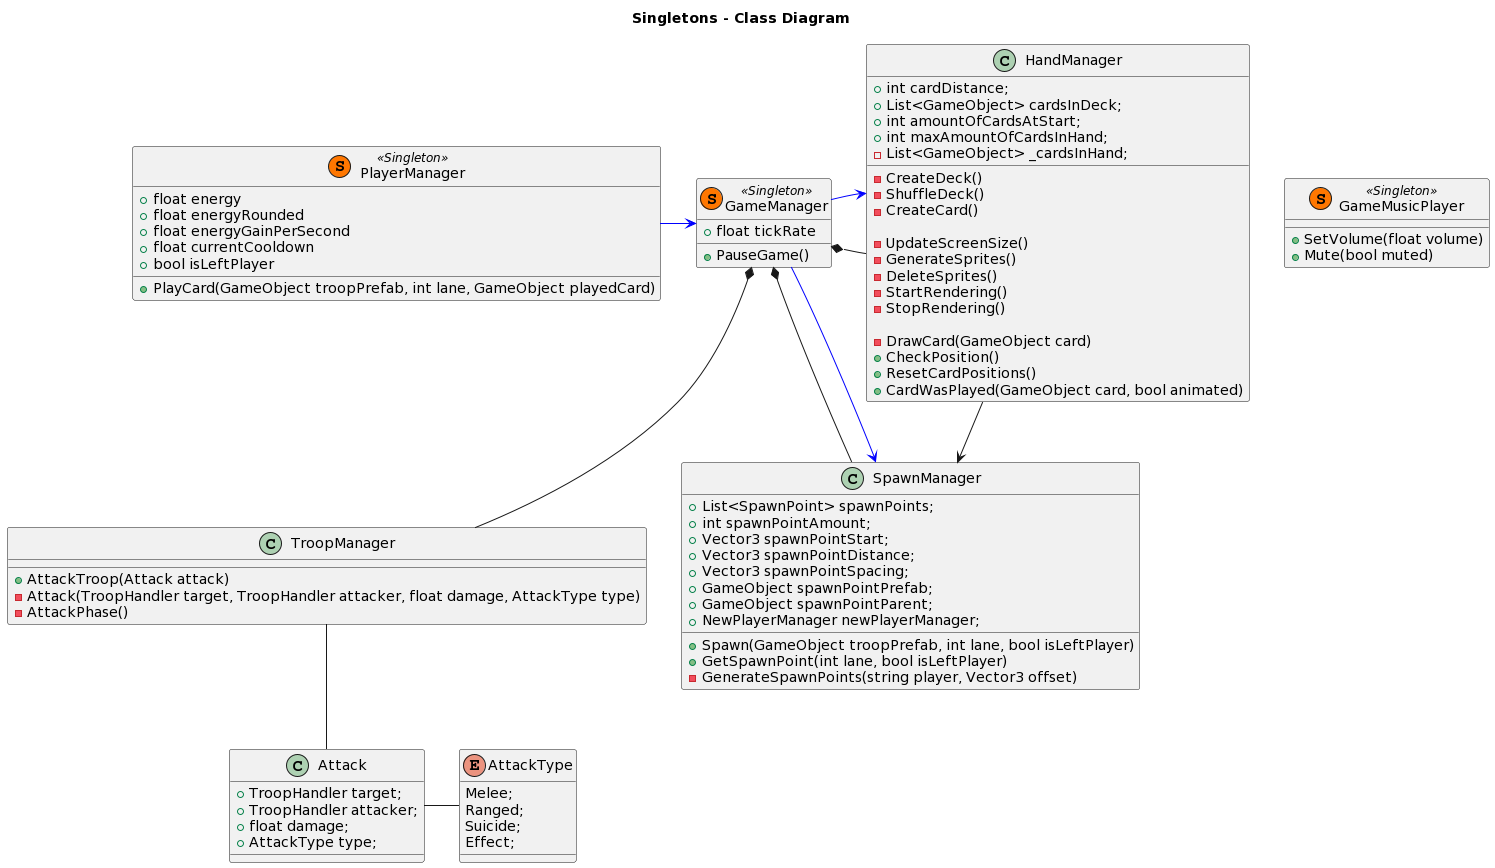
\includegraphics[width=15cm]{resources/Singletons.png} \\
\textit{momentaner Aufbau} \\
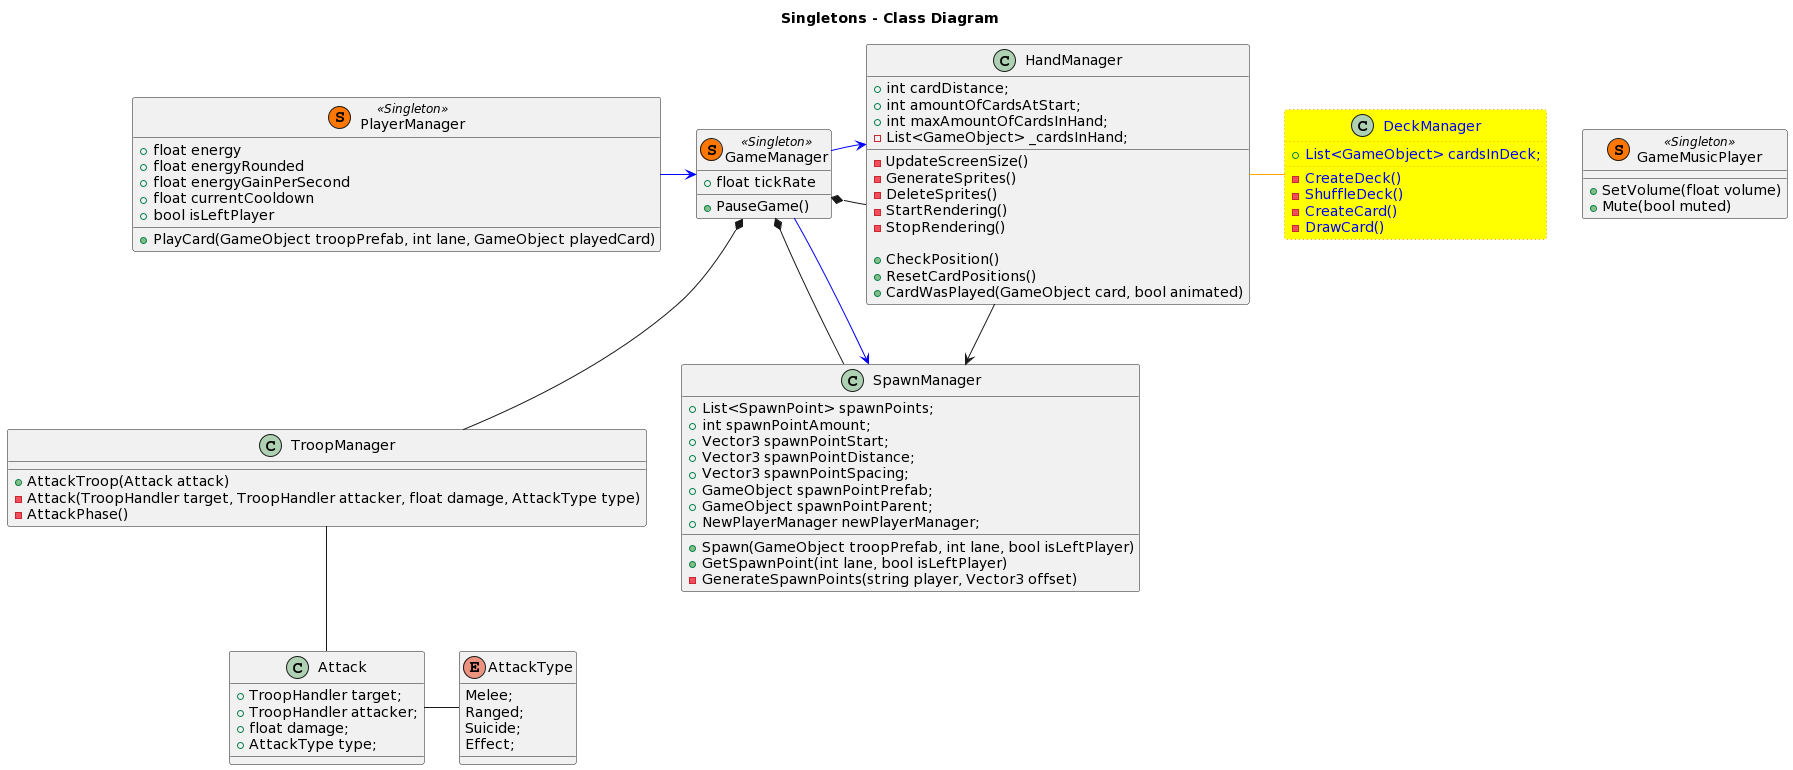
\includegraphics[width=15cm]{resources/Singletons 2.png} \\
\textit{zukünftiger Aufbau}

\section{Truppenarchitektur}
Folgend ist die Abfolge unseres Codes zusehen, falls eine Truppe in die Reichweite einer anderen kommt.
Die erste Abbildung zeigt den Fall einer Nahkampf Truppe und die zweite eine Fernkampftruppe.
Die Suizidtruppe ist gleich aufgebaut wie die Nahkampf Truppe, wobei diese sich einfach selbst zerstört nach dem Angriff. \\
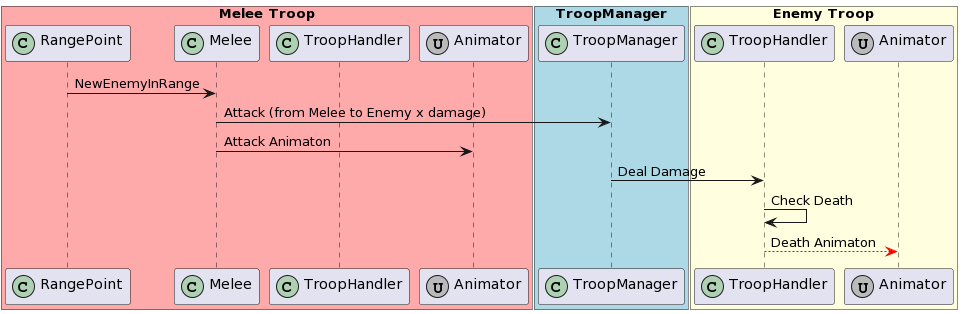
\includegraphics[width=16cm]{resources/MeleeAttacks.png} \\
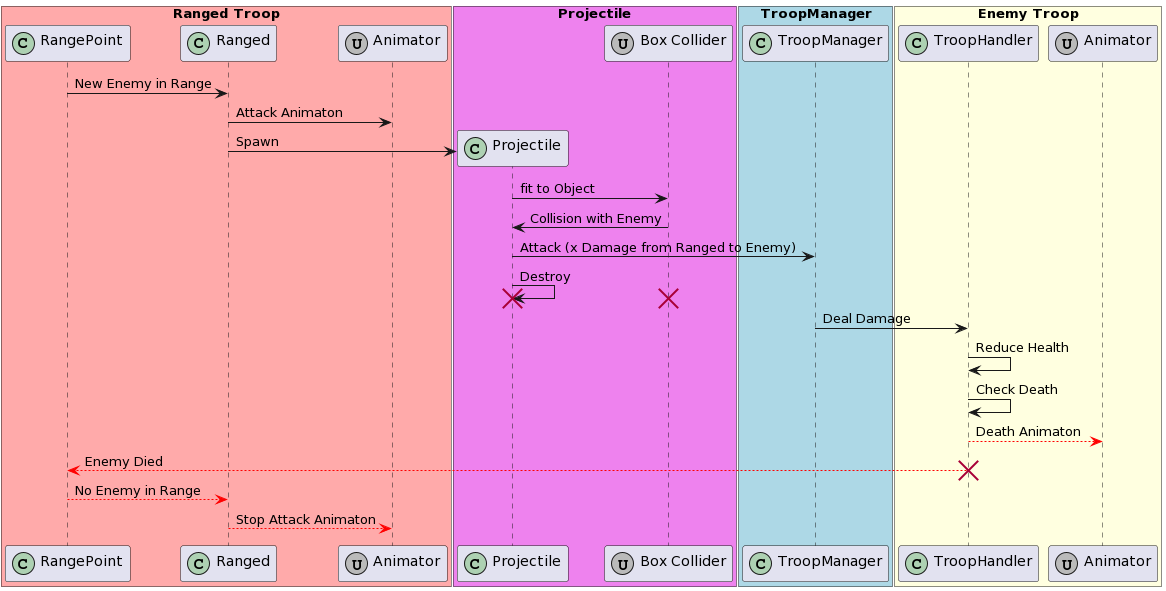
\includegraphics[width=16cm]{resources/RangedAttacks.png} \\
Folgend ist die Selbstzerstörung des Projektils abgebildet, falls die Truppe in Reichweite stirbt und das Projektil nichts trifft \\
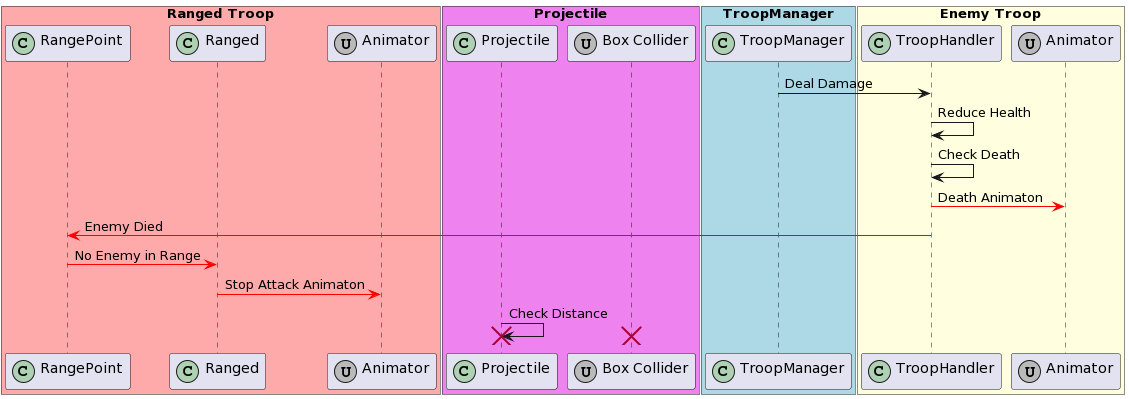
\includegraphics[width=16cm]{resources/Projectile.png} \\

\section{Gift}
Folgend ist die Sequenz abgebildet, falls eine Giftige Truppe angegriffen wird. \\
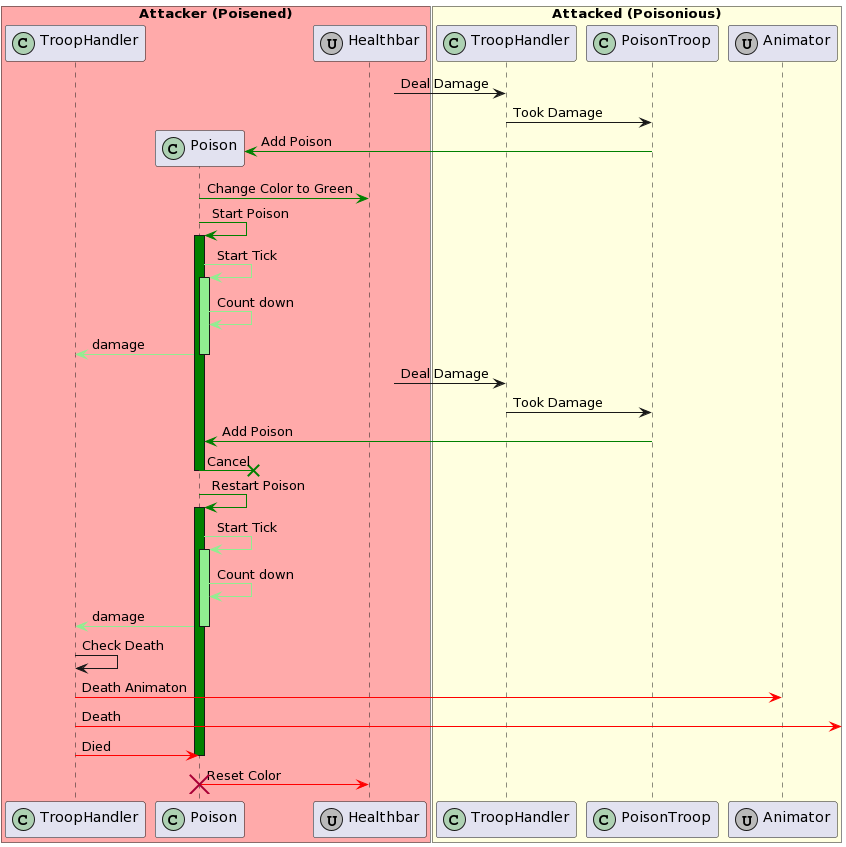
\includegraphics[width=16cm]{resources/Poison.png} \\


\section*{github file system / source / version control}
\url{https://www.youtube.com/watch?v=IQT37uwpcg4}